\section{Introduction}

A business rule articulates some aspect of the expected functional behavior (or
a \textit{requirement}) of an enterprise application. Here is a simple business
rule that determines how an invoice total is determined in a billing
application (specifically, \texttt{jbilling}~\cite{jbilling}):
%
\begin{quote}
{\small
	
The \textit{Balance Type} of a customer affects how invoice total is computed;
it can be one of the following:

\textit{None}: The customer's account will not hold a balance; instead all
charges accrued in an order will be included in the next invoice;
	
\textit{Credit}: The customer's account may accrue charges up to the set credit
limit.  Charges will automatically be paid from the users credit pool until the
set limit is reached.  Users are responsible for paying their credit debt as
well as any overages.

}
\end{quote}	
%
We will examine this rule closely later; for now, suffice it to say that the
requirements of an enterprise system are typically captured by a large number
(often, hundreds) of business rules such as the one above.

It is reasonable to expect functional testing of an enterprise system to
\textit{cover} its business rules, which is to say, testing would exercise all
distinct scenarios described in each business rule.  For example, in the
preceding rule, one of the scenario to be exercised is that a customer's balance
type is credit, and that the order amount exceeds the customer's credit limit.
A test that exercises this scenario would set up a customer with the balance
type as \textit{credit} as well as a certain credit limit (say, \textit{100}),
create an order and add items to the order to bring the total to an amount (say,
\textit{120}) that exceeds the credit limit for that customer, and finally
create an invoice for that order and verify the invoiced amount.
%Figure~\ref{fig:jbilling-flow} illustrates this flow.  
Although the values
\textit{credit}, \textit{100}, and \textit{120} can be identified just from this
rule (by constraint solving), identifying a test sequence is also important to
apply those values at the right fields on the appropriate
screens in the application.
%\footnote{Not all fields on the screens in
%  Figure~\ref{fig:jbilling-flow} are constrained from the point of view of
%  exercising a particular scenario, but the application might still demand
%  sensible values for them. The tester is expected to make these up.}

%\begin{figure*}
%\centering
%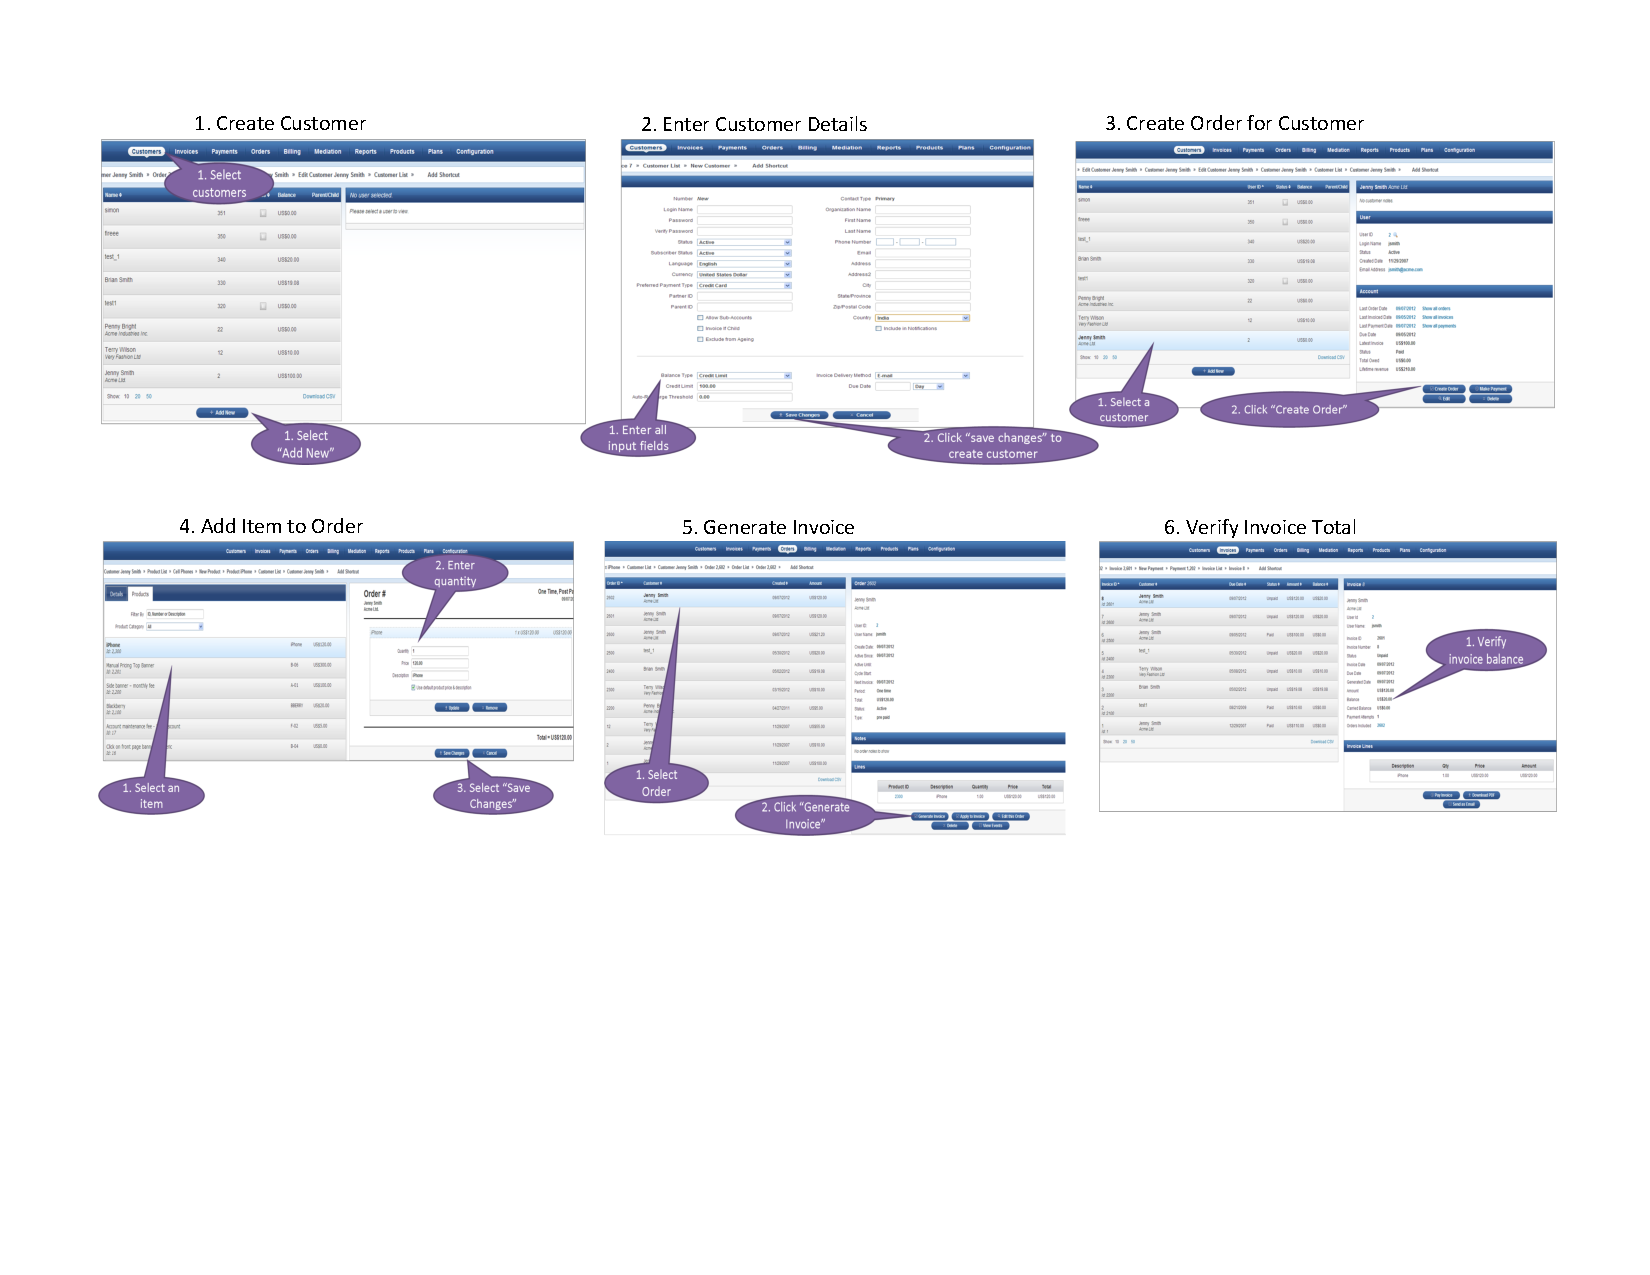
\includegraphics[trim=47 210 35 50,clip,width=\textwidth]{figs/jbilling-flow}
%\vspace*{-10pt}
%\caption{Test sequence for exercising a business rule from the
%  \subject{jBilling} application.}
%\vspace*{-7pt}
%\label{fig:jbilling-flow}
%\end{figure*}

It requires a carefully thought-out test scenario, \ie a sequence of test steps
as well as associated test data, \ie values to be entered in the relevant test
steps to exercise a business rule, or a scenario thereof.  Without systematic
test creation, testers may end up creating multiple tests that exercise the same
business rule, or a scenario thereof, over and over again without any additional
benefit (especially if they are incentivised by the number of tests created
rather than quality of the created tests), and more problematically, may neglect
to create tests for some other business rules.

In practice, due to time pressures, testers are more often ad-hoc than
methodical in creating test scenarios and test data.  One part of the problem is
that a realistic system can have hundreds of business rules written in plain
text, and it is difficult to get a global view of how the rules together
describe the application behavior.  A related part of the problem is that it may
need complex reasoning to piece together test sequences that cover each
scenario.  The net result is that, despite a lot of resources spent in testing,
bugs still escape into field.

\hyphenation{non-prog-ram-mers}

Our vision is to make testing of enterprise software more tool-based, by
adapting technology developed for automated and systematic test generation for
programs. In this vision, business rules would be written in a structured
notation that allows mechanized analysis.  Special editors could be created
to enable non-programm\-ers to capture business rules in a structured notation;
this is an independent challenge in \textit{end-user} programming.  A tool would
validate business rules and point out any ambiguities or omissions that it can
detect.  After the business rules pass validation, another tool would generate
test sequences and test data to exercise the application thoroughly as well as
without redundancies.

We have built a system to partially fulfil this vision.  In the rest of the
introduction, we give an overview of our system, describe some of the challenges
in automating test generation for covering business rules, and summarize our
results.

%Randomly generated test data cannot be expected to suffice for enterprise
%applications with complex rules. Also, systematic test-generation approaches
%based on program analysis (\eg \cite{Emmi:2007,Li:2010,Marcozzi:2012,Pan:2011})
%cannot be expected to tackle enterprise applications, which use a mix of
%multiple language and database technologies in their implementation. Moreover,
%these techniques are directed toward attaining simple forms of code coverage,
%such as statement or branch coverage, rather than coverage of complex business
%rules.

\subsection{An Overview}

Enterprise systems of interest to us are transaction-oriented, which means that
they consist of a set of transactions or operations (\eg create a customer, add
an item to an order, and so on) that operate on databases.  A business rule
applies to a particular operation supported by the system.  Formally, a business
rule describes the relation between the database state before and after the
operation.  Figure~\ref{fig:invoice} shows formalization of the business rule
quoted informally at the beginning of this section.  It says that the operation
refers to an invoice record, \subject{inv}, and modifies specific attributes of
\subject{inv}.  There are three scenarios that occur in this rule.  The first
scenario applies when the customer to which the invoice refers has balance type
\subject{None}; the \textit{precondition} is shown on the left of the first
arrow.  Note that the invoice has references to the customer to which this
invoice pertains and an order created in the system; in a relational database,
these would be foreign keys in the customer and order tables.  The second
scenario applies when the customer has balance type \subject{Credit} and the
credit limit is sufficient to cover the order total.  The third scenario applies
when the customer has balance type \subject{Credit}, but the order total exceeds
the credit limit.  In each scenario, the effect of the operation is to compute
invoice total and update the customer's residual credit limit; this effect, or
\textit{postcondition}, is shown to the right of the arrow.  Note that business
rules refer to the state observable at transaction boundaries; intermediate
program states encountered in the implementation while a transaction is in
process, are not important to business rules.

\begin{figure}
\centering
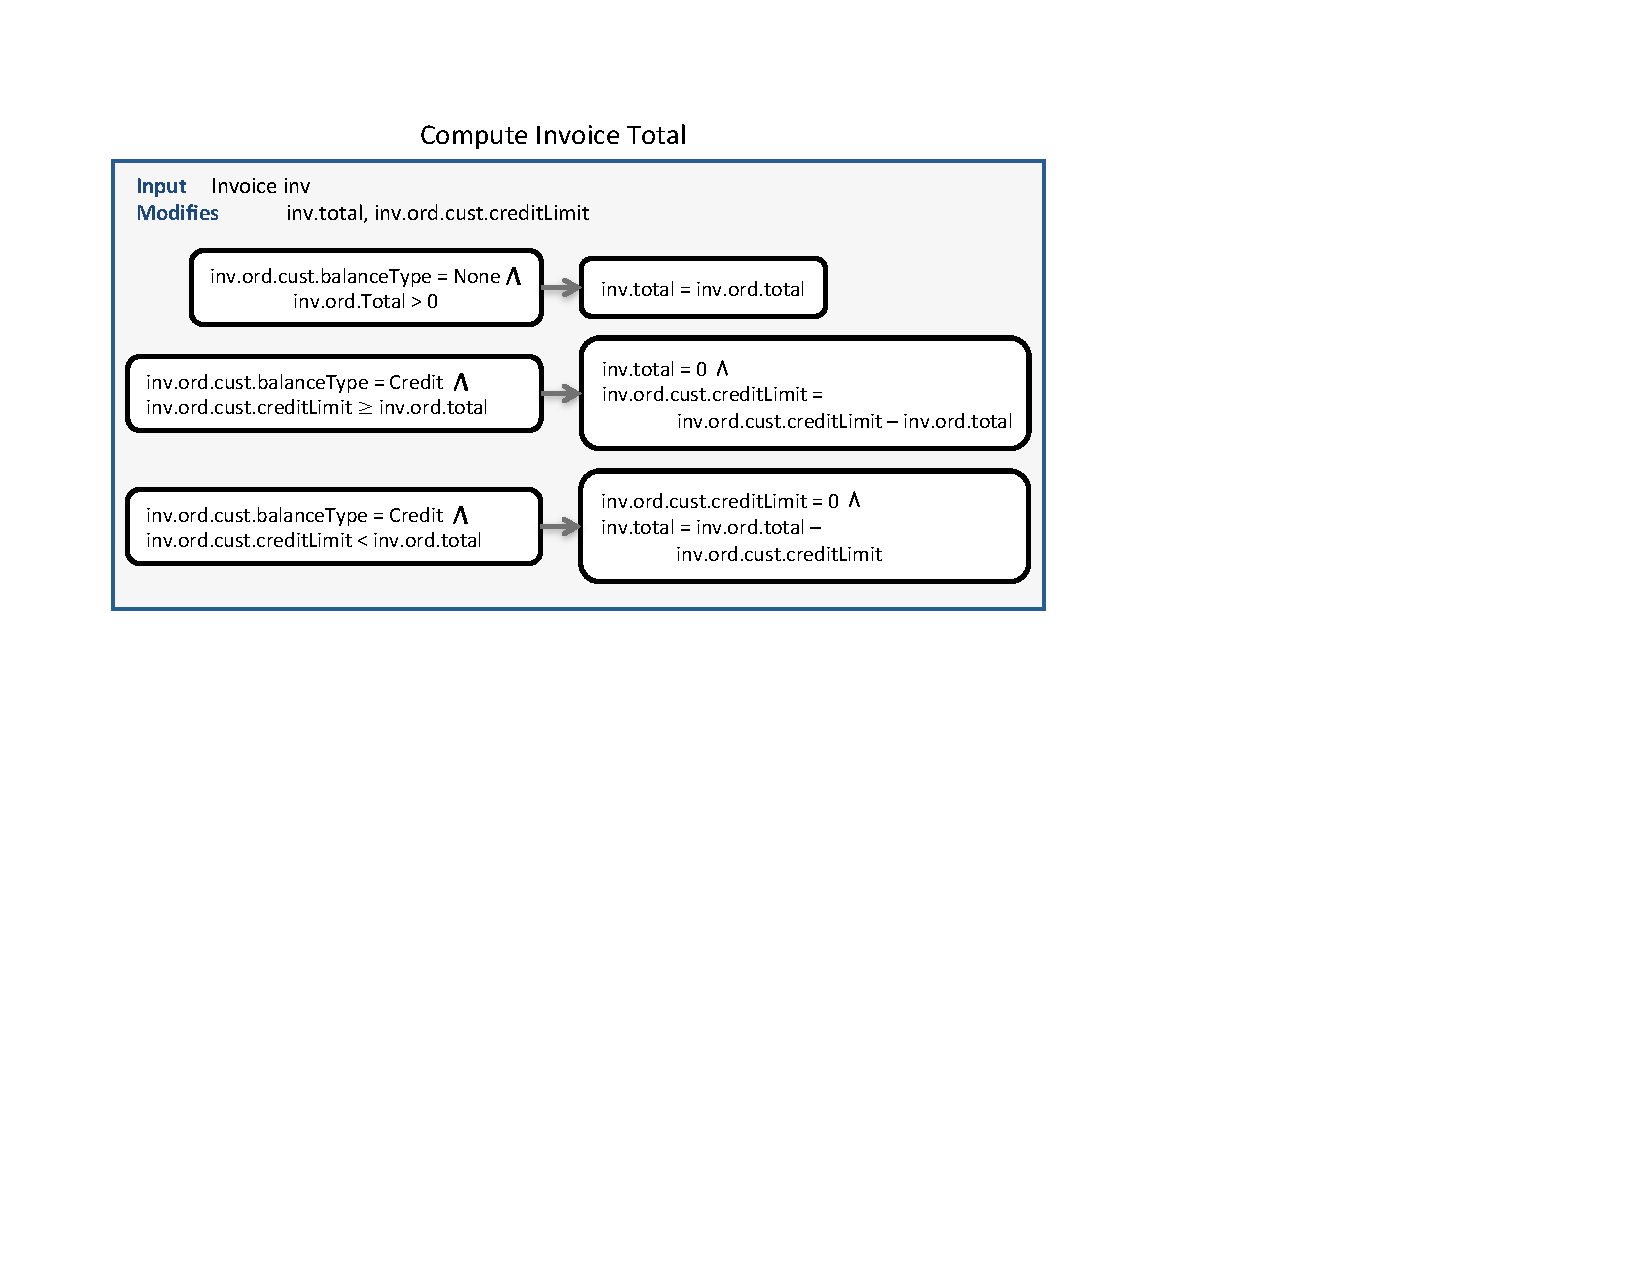
\includegraphics[trim=55 320 286 54,clip,width=\columnwidth]{figs/invoice}
\vspace*{-18pt}
\caption{Business rule for computing invoice amount.}
\label{fig:invoice}
\end{figure}

Covering a business rule means to exercise each of its constituent scenarios,
referred henceforth as \textit{rule parts}.  To cover the three rule parts shown
in Figure~\ref{fig:invoice}, it is necessary to create (separately) each of the
three preconditions and, in each case, verify that the postcondition holds after
the operation has completed.  This brings us to the main difficulty in creating
tests: appropriate database state, such as a customer with a certain balance
type and an order with a certain amount, needs to be established before any of
these scenarios can be exercised.  In the \texttt{jbilling} application's web interface,
it requires entering appropriate data step-wise in six distinct web pages to be able to
bring the state of the application at which these rule parts can be exercised.
%We showed in
%Figure~\ref{fig:jbilling-flow} the steps that would be required to create these
%preconditions.  
How can we identify these steps, and the data to~be entered in
each of the steps, automatically to cover a rule part?

Our observation is that the steps that are required to drive the database state
to a desired precondition are carried out by operations, and those operations
too would have rules that specify their functionality.  (In \texttt{jbilling}, each
operation is triggered by entering appropriate data and clicking on ``submit'' on
a web page specific to that operation.) We could then use
business rules as ``state transformers'' and piece together a sequence of
operations to arrive at a desired state.  The advantage of looking at business
rules as state transformers is that we can adapt the technology developed for
test generation on \textit{programs} for the problem at hand.\footnote{We
  clarify, though, that business rules are themselves not executable programs;
  rather they only are an abstract description of the functionality of a
  program.}  The disadvantage of relying on business rules to act as state
transformers is that they need to be specified to a certain level of detail for
them to work out as state transformers; this is generally not a big
problem---practioners tend to write business rules with an intention to be
complete---but their intended use as input to test generation process does
increase expectations from the rules and, therefore, from the analysts who write
them.

\subsection{Our Approach and Results}

At a high level, the idea is to use backward analysis to piece together a
sequence of operations to arrive at a desired state.  We look for an operation
whose business rule has a rule part whose postcondition would imply the desired
precondition.  Such an operation, if executed in a way that the specific rule
part applies, would establish the desired state.  The operation may require some
user-provided values, but may partially rely on prior database state. The
process is repeated until no prior database state is assumed---that is, all the
database state is established by operations identified in the process.

Consider the second rule part shown in Figure~\ref{fig:invoice}. To satisfy the
precondition of the rule part, a customer with balance type \subject{Credit},
and an associated credit limit, needs to be created first. Then, an order whose
total does not exceed the customer's credit limit needs to be generated, which
involves adding items with suitable prices to the order. Only after this state
has been set up, the operation for invoice generation can be invoked. An
operation sequence and test data (we explain the notation in
Section~\ref{sec:approach}) that achieves this is:

\vspace*{-4pt}%
{\scriptsize
\begin{alltt}
 State st; BalanceType bt = Credit; int crLimit = 100, price = 20;
 Customer cust = CreateCustomer(st, bt);
 Customer cust1 = AddCreditLimit(cust, crLimit);
 Order ord = CreateOrder(cust1);
 Item item = CreateItem(int price);
 Order ord1 = AddItemToOrder(ord, item);
 Invoice inv = GenerateInvoice(ord1);  
\end{alltt}}%
\vspace*{-5pt}

The idea of backward traversal is definitely not novel; it is reminiscent of
weakest preconditions.  Our contribution is to make this idea work in the
context of business rules.  In general, the space of possible operation
sequences can be large, in which only a few sequences cover the target rule
part. Thus, the challenge is to search this space soundly, but efficiently in a
goal-driven manner. Specifically, our technique builds the sequence
incrementally using constraint solving. If the logical formula for a sequence is
not satisfiable, it extracts the unsatisfied core of the formula and constructs
new candidate sequences by considering only those operations and rule parts
whose postconditions are compatible with the unsatisfied core. In this way---and
using additional optimizations---the technique can prune out large parts of the
search space and efficiently narrow down to the covering sequences.

The sequencing of operations done by our algorithm is also reminiscent of the AI planning 
problem [18] where actions with pre- and postconditions are sequenced by a planner 
algorithm using either forward or backward chaining. We discuss the connection
in the related work section; in brief, the algorithms for planning would have to
be fortified with the same kinds of optimizations as mentioned above to be practical
for our use.

An important ingredient of our approach is a notation for capturing business rules 
formally, which enables
mechanized analysis for test generation. Moreover, prior to test generation,
formally specified rules can be checked for consistency and completeness
properties.  The notation is designed to be natural for use by architects, 
and while there is concern of a learning curve whenever a notation has to be adopted,
the industry as a whole has been moving towards structured rule description
languages (e.g. JBoss~\cite{JBoss}, ILOG~\cite{ILog}, 
and RuleML~\cite{RuleML}; see Section~\ref{sec:model}).  We believe the payoff by way 
of consistency checks and automatic test coverage would further spur adoption of structured rule languages.

We have implemented a prototype system, which includes a business rule editor
(an Eclipse plug-in) and automated analyses for rule checking and test
generation. Our preliminary results illustrate the promise of the approach: for
77~rule parts, modeled from three applications, our technique generated covering
sequences and test data for 99\% of the rule parts and missed only one rule part
(which could not be covered because of limitations of the underlying constraint
solver). By comparison, a technique that performs exhaustive (unguided) search
could cover 74\% of the rule parts, although it explored substantially more
candidate sequences than our technique.

%\paragraph*{Contributions}
The contributions of this paper are as follows:
\begin{itemize}[noitemsep]
\item We describe a notation for describing business rules formally, and articulate
  a set of well-formedness properties that can be checked mechanically. We have 
  also developed an Eclipse plugin for our rule language.
\item We describe an algorithm that can mechanically construct test sequences
  that exercise the business rules of a model. The algorithm uses a
  novel optimization to prune the search space. We have implemented
  the algorithm in a tool called \tool{}.
\item To evaluate our approach, we have formalized the business rules
  of three enterprise systems and used \tool{} to generate test
  sequences. Using our approach we are able to generate tests for 99\%
  of the rule parts.
\end{itemize}

%In Section~\ref{sec:model}, we describe our notation for modeling business
%rules and present four well-formedness properties of
%models. In Section~\ref{sec:example}, we present the running example
%model, JBilling. In Section~\ref{sec:approach} we describe our approach including several
%optimizations. In Section~\ref{sec:eval} is the experimental evaluation using
%our implementation \tool{} and in Section~\ref{sec:related} we discuss related
%research.   
